\subsubsection{Memory Access Patterns}
\par{Data access pattern in kernel code is shown in figure \ref{nbodyMAP}.}

\begin{figure}[!h]
    \centering
    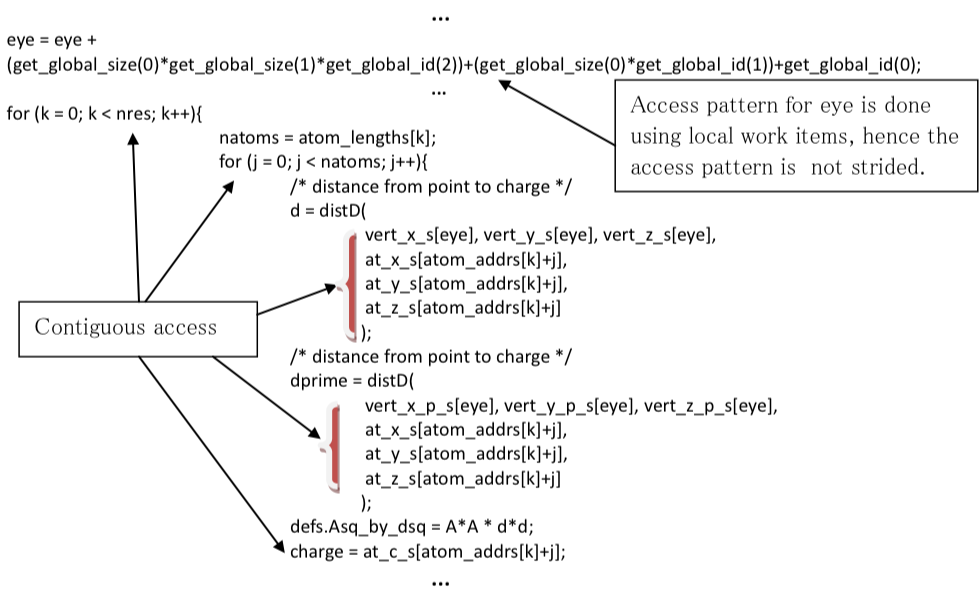
\includegraphics[width=0.8\textwidth]{figures/nbodyMAP.png}
    \caption{Data access pattern in NBody Kernel.}
    \label{nbodyMAP}
\end{figure}

\par{To test the memory access pattern of the code, the index 
    number through which the various array elements are accessed
    upon each iteration of the loop, were printed (figure \ref{nbodyMAP}). 
    The results showed that the atomic data was being accessed in a 
    serialized (1,2,3,4 ...) pattern, by all work items simultaneously. 
    This aspect explains the efficient use of cache memory by the code and 
    is backed up by the very high L1 hit ratio results (figure \ref{nbodyL1}) 
    shown by the VTune profiler.}

\begin{figure}[!h]
    \centering
    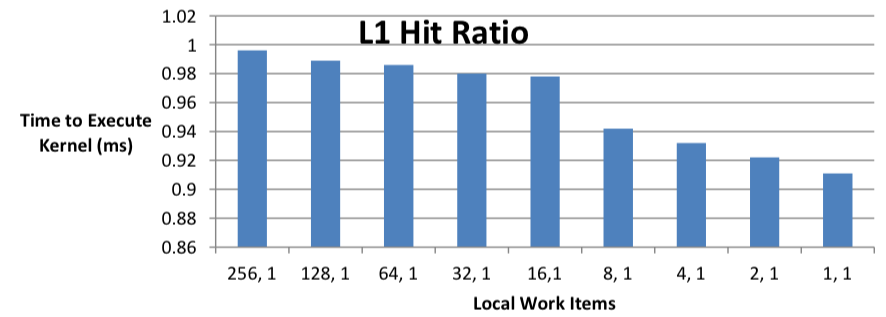
\includegraphics[width=0.8\textwidth]{figures/nbodyL1.png}
    \caption{L1 Hit Ratio Xeon Phi NBody.}
    \label{nbodyL1}
\end{figure}

\par{Running the same kernel using the same input file 
    (bio molecule and vertex locations) on the same architecture resulted 
    in the same output (electrostatic potential for each vertex) on every run, 
    regardless of work item size. This proves that the code is stable.}

\par{However, upon comparing results for tests under similar settings for 
    all of the 3 different architectures, resulted in variations of the 
    decimal numbers for 10\^-4 and below. Please look at table above.
    One possible theory for this is that since the architectures have different 
    types of parallelism, there is a potential issue of order of aggregating 
    results. As OpenCL is providing portability, the order of calculating 
    floating point numbers would have changed which ultimately resulting in 
    such errors. The order can make a significant difference on the result 
    when aggregating floating point numbers ({\color{red}cite})}

\par{This shows that the Open Dwarfs implementation is 
    more focused on performance rather than experimental accuracy. 
    It is also important to point out that the above are just theories 
    and further analysis and testing needs to be done to confirm them.}

\subsubsection{Factors which contribute to inefficiencies in the code}
\par{The value of r (distance from the point of observation to the ``centre'') 
    passed to the kernel code is crucial, as it decides (using conditionals) 
    the type of calculation to be done on the point of interest. 
    The value of r is compared against rprime (Threshold for the 
    ion exclusion radius) and A. If r > rprime, then the atoms are 
    considered as distant components. If r<A, then 0 < dist\_to\_surf <= ion\_excl\_rad. 
    Otherwise the point is considered to be on the surface (a vertex) of the 
    molecule. With the tests that have been run on this code, the preset value 
    for p (perpendicular distance of the vertex point from the surface of 
    the molecule) was 0.0. This resulted in only one set of conditionals 
    ever being executed in the code. This is a possible case for 
    inefficiency.}

\par{Since kernel code is compiled at run time, there is an overhead
    with the if else condition. In this N Body kernel, only one set of 
    if statements are always executed. Since the other if else statements 
    are not being used, they are causing a certain amount of overhead 
    every time.}

\subsubsection{Opportunity for Optimisation}
\par{The n body implementation in OpenDwarfs calls the kernel multiple 
    times based on the number of vertices in the data file to be processed. 
    This also depends on the number of global work items.}

\par{No of times Kernel is called = No of Vertices/(GWI in X*GWI*Y)}

\par{One possible optimisation might be to choose the global work 
    item size such that the total number of work items equals 
    to or exceeds the number of vertices. In this way the kernel 
    code will not have to be called multiple times saving the host code to 
    execute the kernel enqueing numerous times.}

\par{Therefore dependent on the size of the input file 
    you should accordingly adjust the Global work item sizes. 
    Upon testing on the different hardware, the test results 
    are not impacted.}

\subsubsection{NULL and Personal Experience with OpenCL}
\par{OpenCL has an in-built feature which allows the programmer to let the 
    compiler decide the local work item sizes based on your selected global 
    work items and the kernel code which is executed. Tests were taken to 
    try and see the efficiency of this feature and the results were positive. 
    The NULL feature is able to come quite close to the optimal work item 
    size in all three hardware test instances*. This can be seen on the 
    graphical results for the different architectures on the previous pages. 
    This is a good feature for OpenCL as it removes the need to benchmark 
    the kernels for the best result. Of course the optimal performance might 
    not be achieved but, as the results show, if there is not enough time to 
    fine-tune the work group sizes, this feature can handle it well.}

\par{Unable to see values for local work items on GPU since it 
    ran on OpenCL1.0 which did not have support for printf 
    within kernel. Upon testing NULL, total kernel execution 
    time was 54794.31149 ms, which is very close to optimal 
    performance for Capsid molecule.}


